\documentclass[14pt,a4paper,report]{report}
\usepackage[a4paper, mag=1000, left=2.5cm, right=1cm, top=2cm, bottom=2cm, headsep=0.7cm, footskip=1cm]{geometry}
\usepackage[utf8]{inputenc}
\usepackage[english,russian]{babel}
\usepackage{indentfirst}
\usepackage[dvipsnames]{xcolor}
\usepackage[colorlinks]{hyperref}
\usepackage{listings} 
\usepackage{fancyhdr}
\usepackage{caption}
\usepackage{amsmath}
\usepackage{latexsym}
\usepackage{graphicx}
\hypersetup{
	colorlinks = true,
	linkcolor  = black
}

\usepackage{titlesec}
\titleformat{\chapter}
{\Large\bfseries} % format
{}                % label
{0pt}             % sep
{\huge}           % before-code


\DeclareCaptionFont{white}{\color{white}} 

% Listing description
\usepackage{listings} 
\DeclareCaptionFormat{listing}{\colorbox{gray}{\parbox{\textwidth}{#1#2#3}}}
\captionsetup[lstlisting]{format=listing,labelfont=white,textfont=white}
\lstset{ 
	% Listing settings
	inputencoding = utf8,			
	extendedchars = \true, 
	keepspaces = true, 			  	 % Поддержка кириллицы и пробелов в комментариях
	language = C,            	 	 % Язык программирования (для подсветки)
	basicstyle = \small\sffamily, 	 % Размер и начертание шрифта для подсветки кода
	numbers = left,               	 % Где поставить нумерацию строк (слева\справа)
	numberstyle = \tiny,          	 % Размер шрифта для номеров строк
	stepnumber = 1,               	 % Размер шага между двумя номерами строк
	numbersep = 5pt,              	 % Как далеко отстоят номера строк от подсвечиваемого кода
	backgroundcolor = \color{white}, % Цвет фона подсветки - используем \usepackage{color}
	showspaces = false,           	 % Показывать или нет пробелы специальными отступами
	showstringspaces = false,    	 % Показывать или нет пробелы в строках
	showtabs = false,           	 % Показывать или нет табуляцию в строках
	frame = single,              	 % Рисовать рамку вокруг кода
	tabsize = 2,                  	 % Размер табуляции по умолчанию равен 2 пробелам
	captionpos = t,             	 % Позиция заголовка вверху [t] или внизу [b] 
	breaklines = true,           	 % Автоматически переносить строки (да\нет)
	breakatwhitespace = false,   	 % Переносить строки только если есть пробел
	escapeinside = {\%*}{*)}      	 % Если нужно добавить комментарии в коде
}

\begin{document}

\chapter{Домашнее задание №2}

\subsubsection{Бояркин 43501/3}

\section{Принцип суперпозиции и принцип гомогенности}

\textbf{Принцип суперпозиции} заключается в том, что реакция системы на несколько одновременно действующих входных воздействия равна сумме реакций на каждое воздействие в отдельности.

Принцип суперпозиции всегда выполняется, если выполняются следующие два условия:

\begin{itemize}
	\item При суммировании любых двух входных сигналов соответствующие выходные сигналы суммируются.
	\item При любом увеличении (уменьшении) входного сигнала без изменения его формы выходной сигнал увеличивается (уменьшается) во столько же раз, также не изменяя своей формы.
\end{itemize}

\textbf{Принцип гомогенности} линейной системы предполагает выполнение условия масштабируемости, то есть при изменении входного сигнала \emph{x} в \emph{k} раз выходной сигнал \emph{y} линейной САУ изменится соответственно в \emph{k} раз.

\section{Свойства прямого и обратного преобразования Лапласа}

Свойства прямого и обратного преобразований Лапласа:

\begin{figure}[h!]
	\centering
	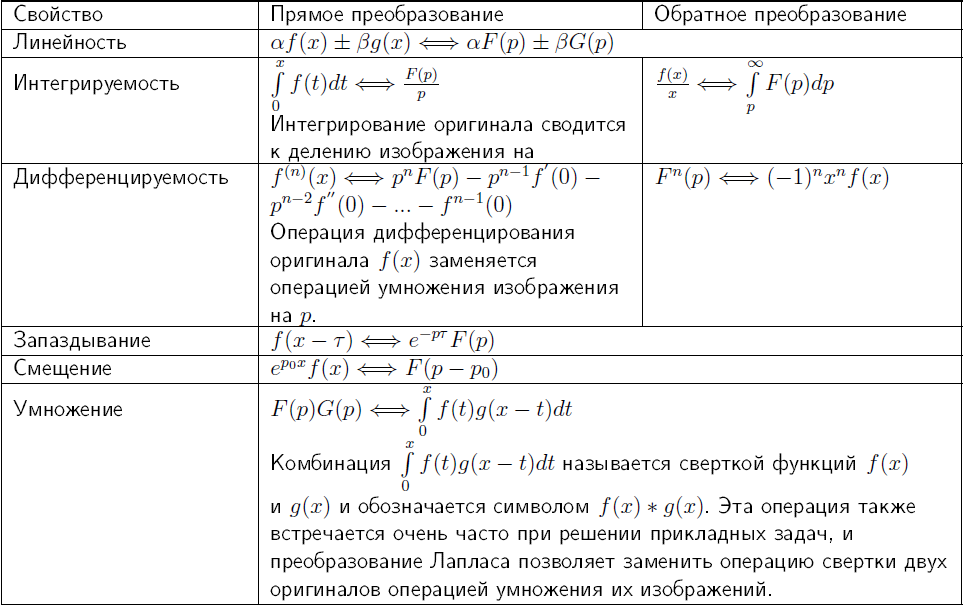
\includegraphics[scale = 0.68]{images/1.png}
	
	\label{table:1}
\end{figure}

\section{Взаимосвязь пяти форм}

Переход от дифференциальных уравнений к передаточной функции осуществляется следующим образом: в первую очередь сводим нелинейные ДУ к линейным по теореме Тейлора. После этого преобразуем его в операторную форму и получим пропорцию, которая и будет являться передаточной функцией: 

$ \sum_{i=0}^{n}a_{i}p^{(i)}\bigtriangleup Y = \sum_{j=0}^{m}b_{j}p^{(j)}\bigtriangleup U \Longleftrightarrow \frac{\bigtriangleup Y(p)}{\bigtriangleup U(p)}=\frac{\sum_{j=0}^{m}b_{j}p^{(j)}}{\sum_{i=0}^{n}a_{i}p^{(i)}} = W(p) $ 

Получение передаточной функции из уравнения объекта управления осуществляется следующим образом: сводим уравнение Коши в операторную форму, после этого получаем однозначным преобразованием передаточную функцию. Стоит отметить что обратное преобразование неоднозначное и многосложное:


\begin{equation*}
	\begin{cases}
		\text{$X'(t)=A X(t) + B U(t)$} \\
		\text{$Y(t)=C X(t)$} \\
		\text{$X(0)=x_{0}$}
	\end{cases}
	\Longleftrightarrow 
	\begin{cases}
		\text{$p X=A X + B U$} \\
		\text{$Y=C X$}
	\end{cases}
	\Longrightarrow
	\text{$Y=C (E p-A) B U=W(p) U$}
\end{equation*}






\end{document}